\section{Polarization ellipse derivation}
\label{sec:deriv_pol_ellipse}
Setting $kz-\omega t=\tau$ in the plane wave equations:
\begin{equation}
\begin{aligned}
    E_x(z, t) = E_{0x}\cos(\tau + \delta_x) \\
    E_y(z, t) = E_{0y}\cos(\tau + \delta_y).
\end{aligned}
\end{equation}
In order to eliminate $\tau$ we write the previous equations as:
\begin{equation}
\begin{aligned}
    \frac{E_x}{E_{0x}} = \cos(\tau)\cos(\delta_x) - \sin(\tau)\sin(\delta_x)\\
    \frac{E_y}{E_{0y}} = \cos(\tau)\cos(\delta_y) - \sin(\tau)\sin(\delta_y).
\end{aligned}
\end{equation}
Multiplying by $\cos(\delta_{x,y})$, $\sin(\delta_{x,y})$ subtracting and using trig. angle difference formulas we get:
\begin{equation}
\begin{aligned}
    \frac{E_x}{E_{0x}}\sin(\delta_y) - \frac{E_y}{E_{0y}}\sin(\delta_x) = \cos(\tau)\sin(\delta_y-\delta_x)\\
    \frac{E_x}{E_{0x}}\cos(\delta_y) - \frac{E_y}{E_{0y}}\cos(\delta_x) = \sin(\tau)\sin(\delta_y-\delta_x).
\end{aligned}
\end{equation}
Squaring and adding these two equations gives:
\begin{equation}
    \left(\frac{E_x}{E_{0x}}\right)^2+\left(\frac{E_y}{E_{0y}}\right)^2-2\frac{E_x E_y}{E_{0x} E_{0y}}\cos \delta =\sin^2 \delta,
\end{equation}
with $\delta=\delta_y-\delta_x$, which is the polarization ellipse equation.

\section{Index ellipsoid procedure}
\label{sec:index_ellipse_proof}
% laser book

\section{Effective permittivity inequality}
\label{sec:bf_proof}
% my papers maybe shorten it a bit or only give outline ...


\section{Transmission minimum of diattenuating linear retarder} % Jan measurement setup
\label{sec:transmission_min}
The setup consists of a linear horizontal polarizer $\hat{T}_{DL}(\psi=0, p_1=1, 0)$, linear diattenuating retarder (waveplate) $\hat{T}_{RDL}(\psi, \Delta, p_1, p_2)$ and another linear horizontal polarizer $\hat{T}_{DL}(\psi=0, p_1=1, 0)$ in the given order. The input is a normalized horizontal linear state $\bm{\mathcal{E}}_{\SI{0}{\degree}}$. The intensity of the output is then simply $I_o=T_{1,1}(T_{1,1})^*$, requiring $0\overset{!}{=}I_o$ we get the following:
\begin{equation}
    0=(p_1c_\psi^2e^{i\Delta/2}+p_2s_\psi^2e^{-i\Delta/2})(p_1c_\psi^2e^{-i\Delta/2}+p_2s_\psi^2e^{i\Delta/2}).
\end{equation}
Simplifying:
\begin{equation}
    \label{eq:trans_min_app}
    -2p_1p_2c_\Delta = p_1^2\left(\frac{c_\psi}{s_\psi}\right)^2 + p_2^2\left(\frac{s_\psi}{c_\psi}\right)^2
\end{equation}
The image of LHS is the interval $\left[-2p_1p_2, 2p_1p_2\right]$ while the image of the RHS is $\left[2p_1p_2, \infty\right)$. This means that equation \ref{eq:trans_min_app} only has a solution when
\begin{equation}
    c_\Delta=-1
\end{equation}
and
\begin{equation}
    2p_1p_2 = p_1^2\left(\frac{c_\psi}{s_\psi}\right)^2 + p_2^2\left(\frac{s_\psi}{c_\psi}\right)^2.
\end{equation}
From the first equation it follows that $\Delta=\pi$ $(\Delta \in [0,\pi])$ and the second equation is solved by:
\begin{equation}
    \label{eq:psi_min}
    \psi = \arctan \sqrt{\frac{p_2}{p_1}},
\end{equation}
that is, the intensity is zero for this $\psi=\psi_{min}$ given by equation \ref{eq:psi_min}, which is what we wanted to show.

\section{Basin-hopping algorithm}
\label{sec:basin_hopping_algo}

Basin-hopping is a stochastic algorithm which is used in global optimization problems and was first developed to solve problems in chemical physics \cite{Wales1997}. It is well suited for the optimization problems presented in this work, since it is an effective algorithm in the case of high dimensional smooth nonlinear loss functions $L(x)$ with multiple optima separated by large barriers \cite{Olson2012, Wu2020}. The algorithm mainly consists of cycling through three steps until some stop criterion is fulfilled. First a perturbation of a candidate solution is performed, then a local search is applied to the perturbed solution and then finally the coordinates are accepted or rejected based on the minimized function value. The associated pseudocode is shown in algorithm \ref{algo_bh}. 

\begin{algorithm}[H]
    \SetAlgoLined
    \SetKwFunction{LOCALSEARCH}{LOCALSEARCH}\SetKwFunction{STOP}{STOP}\SetKwFunction{PERTURB}{PERTURB}
    \SetKwFunction{METROPOLIS}{METROPOLIS}
    \SetKw{KwOr}{or}
    \SetKwData{NS}{not satisfied} \SetKwData{RP}{random initial point in variable space}
    
    $i \leftarrow 0$\;
    $x_i \leftarrow $ \RP\;
    $y_i \leftarrow $ \LOCALSEARCH{$x_i$}\;
    \While{\STOP \NS}{
        $x_{i+1} \leftarrow $ \PERTURB{$y_i$}\;
        $y_{i+1} \leftarrow $ \LOCALSEARCH{$x_i$}\;
        \If{$L(y_{i+1})<L(y_i)$ \KwOr{} \METROPOLIS{$y_{i+1}, y_i$}}{
            $i \leftarrow i+1$\;
        }
    }


\caption{Basin-hopping pseudocode}\label{algo_bh}
\end{algorithm}

Since we can not determine if the global minimum has actually been found for stochastic global optimization problems the \texttt{STOP} criterion is simply a number of iterations. The result is then the lowest minimum found. The additional acceptance criterion \texttt{METROPOLIS} is true with a probability $P(y_{i+1}, y_i)$ given by the following:
\begin{equation}
    P(y_{i+1}, y_i) = \exp\left(\frac{L(y_{i})-L(y_{i+1})}{T} \right),
\end{equation}
where $T$ is known as the temperature and is a user defined parameter which should be set similar to the average function value difference between local minima \cite{ScipyBH}. The \texttt{LOCALSEARCH} step is in our case perfomed by the L-BFGS-B local optimization routine which is a quasi-Newton algorithm and allows the specification of bounds \cite{Byrd1995}. \texttt{PERTURB} is responsible for taking a step in variable space with a stepsize $\tau$ which is another user defined parameter. $\tau$ is an important parameter in Basin-hopping and depends on the optimization problem. The step is chosen uniformly in the region from $x-\tau$ to $x+\tau$, in each dimension. The Python implementation of the algorithm as we use it automatically adjusts the stepsize. Nevertheless, to achieve faster convergence the initial value should be similar to the average separation between local minima in variable space \cite{ScipyBH}. 

% TODO rewrite caption below (done)
\begin{figure}[h]
    \centering
    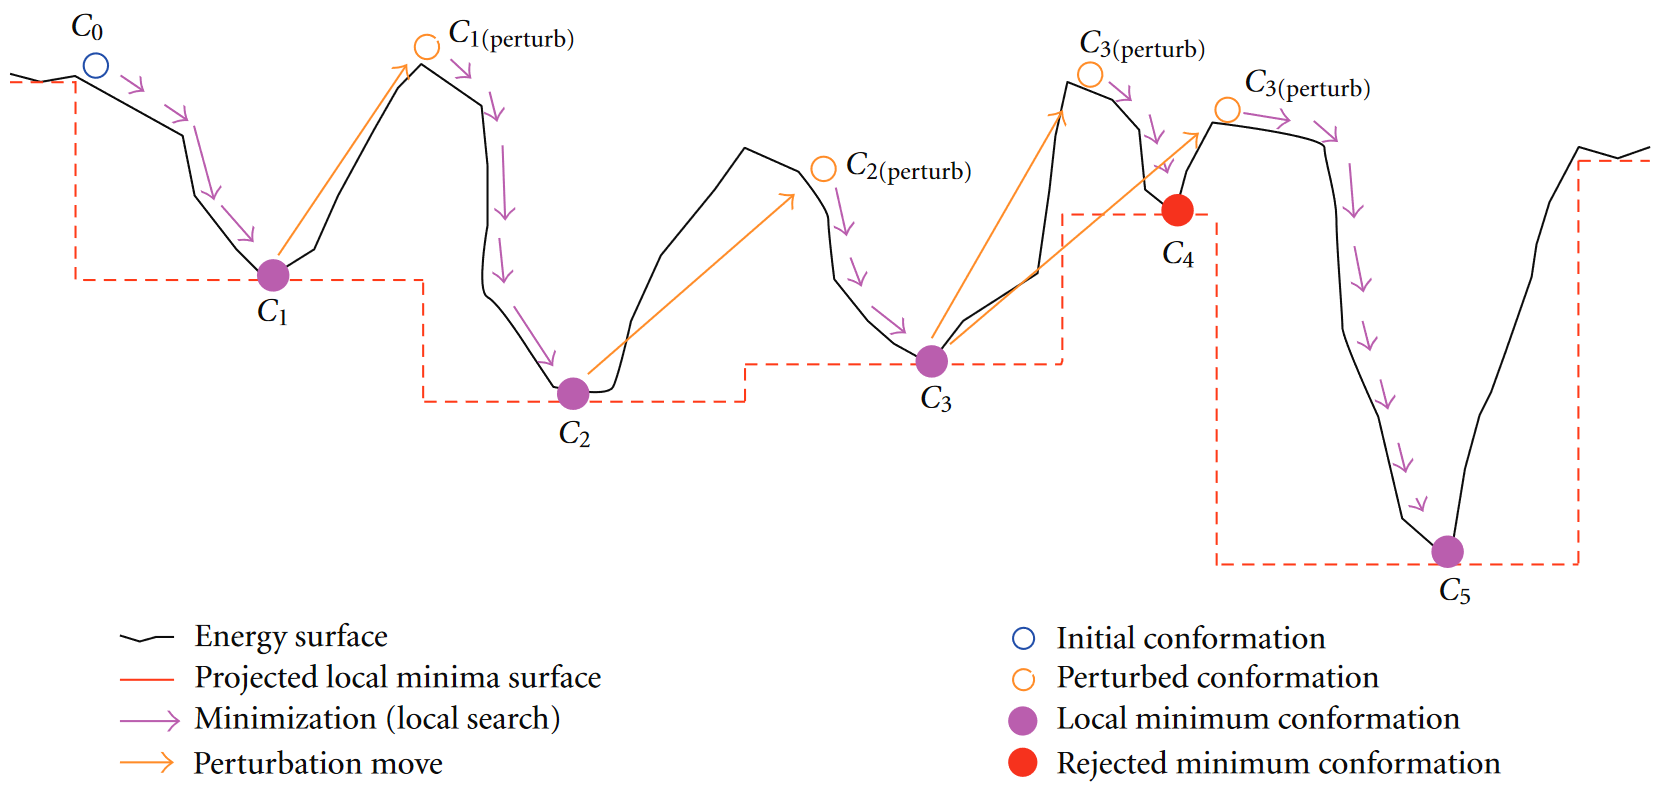
\includegraphics[scale=0.3]{images/7_appendix/bh.png}
    \caption{The Basin-hopping algorithm can be visualized as a transformation of the loss function (black line) into single steps(dotted line). 
    The local optimization routine is illustrated by purple arrows while the random perturbation is represented by yellow arrows. At $C_3$ the perturbation move fails the Metropolis acceptance criterion since the barrier is too high, a new perturbation move to a more favorable position is therefore made. Source: \cite{Olson2012}.}
    \label{fig:Basin-hopping}
\end{figure}

\section{Quartz Sellmeier fit}
\label{sec:sellmeier}
Crystalline Quartz values and stuff

\section{Alternative quarter wave loss function}
\label{sec:int_loss_function}


